% (find-LATEX "2020-1-C2-VS.tex")
% (defun c () (interactive) (find-LATEXsh "lualatex -record 2020-1-C2-VS.tex" :end))
% (defun C () (interactive) (find-LATEXsh "lualatex 2020-1-C2-VS.tex" "Success!!!"))
% (defun D () (interactive) (find-pdf-page      "~/LATEX/2020-1-C2-VS.pdf"))
% (defun d () (interactive) (find-pdftools-page "~/LATEX/2020-1-C2-VS.pdf"))
% (defun e () (interactive) (find-LATEX "2020-1-C2-VS.tex"))
% (defun u () (interactive) (find-latex-upload-links "2020-1-C2-VS"))
% (defun v () (interactive) (find-2a '(e) '(d)))
% (defun cv () (interactive) (C) (ee-kill-this-buffer) (v) (g))
% (find-pdf-page   "~/LATEX/2020-1-C2-VS.pdf")
% (find-sh0 "cp -v  ~/LATEX/2020-1-C2-VS.pdf /tmp/")
% (find-sh0 "cp -v  ~/LATEX/2020-1-C2-VS.pdf /tmp/pen/")
%   file:///home/edrx/LATEX/2020-1-C2-VS.pdf
%               file:///tmp/2020-1-C2-VS.pdf
%           file:///tmp/pen/2020-1-C2-VS.pdf
% http://angg.twu.net/LATEX/2020-1-C2-VS.pdf
% (find-LATEX "2019.mk")
% (find-C2-aula-links "2020-1-C2-VS" "vs" "vs")

\documentclass[oneside,12pt]{article}
\usepackage[colorlinks,citecolor=DarkRed,urlcolor=DarkRed]{hyperref} % (find-es "tex" "hyperref")
\usepackage{amsmath}
\usepackage{amsfonts}
\usepackage{amssymb}
\usepackage{pict2e}
\usepackage[x11names,svgnames]{xcolor} % (find-es "tex" "xcolor")
%\usepackage{colorweb}                 % (find-es "tex" "colorweb")
%\usepackage{tikz}
%
% (find-dn6 "preamble6.lua" "preamble0")
%\usepackage{proof}   % For derivation trees ("%:" lines)
%\input diagxy        % For 2D diagrams ("%D" lines)
%\xyoption{curve}     % For the ".curve=" feature in 2D diagrams
%
\usepackage{edrx15}               % (find-LATEX "edrx15.sty")
\input edrxaccents.tex            % (find-LATEX "edrxaccents.tex")
\input edrxchars.tex              % (find-LATEX "edrxchars.tex")
\input edrxheadfoot.tex           % (find-LATEX "edrxheadfoot.tex")
\input edrxgac2.tex               % (find-LATEX "edrxgac2.tex")
%
%\usepackage[backend=biber,
%   style=alphabetic]{biblatex}            % (find-es "tex" "biber")
%\addbibresource{catsem-slides.bib}        % (find-LATEX "catsem-slides.bib")
%
% (find-es "tex" "geometry")
\usepackage[a6paper, landscape,
            top=1.5cm, bottom=.25cm, left=1cm, right=1cm, includefoot
           ]{geometry}
%
\begin{document}

\catcode`\^^J=10
\directlua{dofile "dednat6load.lua"}  % (find-LATEX "dednat6load.lua")

% %L dofile "edrxtikz.lua"  -- (find-LATEX "edrxtikz.lua")
% %L dofile "edrxpict.lua"  -- (find-LATEX "edrxpict.lua")
% \pu

% «defs»  (to ".defs")
% (find-LATEX "edrx15.sty" "colors-2019")
\long\def\ColorRed   #1{{\color{Red1}#1}}
\long\def\ColorViolet#1{{\color{MagentaVioletLight}#1}}
\long\def\ColorViolet#1{{\color{Violet!50!black}#1}}
\long\def\ColorGreen #1{{\color{SpringDarkHard}#1}}
\long\def\ColorGreen #1{{\color{SpringGreenDark}#1}}
\long\def\ColorGreen #1{{\color{SpringGreen4}#1}}
\long\def\ColorGray  #1{{\color{GrayLight}#1}}
\long\def\ColorGray  #1{{\color{black!30!white}#1}}
\long\def\ColorBrown #1{{\color{Brown}#1}}
\long\def\ColorBrown #1{{\color{brown}#1}}

\long\def\ColorShort #1{{\color{SpringGreen4}#1}}
\long\def\ColorLong  #1{{\color{Red1}#1}}

\def\frown{\ensuremath{{=}{(}}}
\def\True {\mathbf{V}}
\def\False{\mathbf{F}}
\def\D    {\displaystyle}

\def\drafturl{http://angg.twu.net/LATEX/2020-1-C2.pdf}
\def\drafturl{http://angg.twu.net/2020.1-C2.html}
\def\draftfooter{\tiny \href{\drafturl}{\jobname{}} \ColorBrown{\shorttoday{} \hours}}

% (find-angg ".emacs" "c2q192")


%  _____ _ _   _                               
% |_   _(_) |_| | ___   _ __   __ _  __ _  ___ 
%   | | | | __| |/ _ \ | '_ \ / _` |/ _` |/ _ \
%   | | | | |_| |  __/ | |_) | (_| | (_| |  __/
%   |_| |_|\__|_|\___| | .__/ \__,_|\__, |\___|
%                      |_|          |___/      
%
% «title»  (to ".title")

\thispagestyle{empty}

\begin{center}

\vspace*{1.2cm}

{\bf \Large Cálculo 2 - 2020.1}

\bsk

Instruções para a VS --- que vai ser

um trabalho em vídeo ao invés de uma prova

\bsk

Eduardo Ochs - RCN/PURO/UFF

\url{http://angg.twu.net/2020.1-C2.html}

\end{center}

\newpage

O tema \ColorRed{básico} deste trabalho vai ser como calcular esta
integral:
%
$$\intx{\sqrt{1-x^2}}$$

Ela é bem difícil, e quase todo mundo erra tanto nas contas quanto
como nos argumentos geométricos das 20 primeiras vezes que tenta
calculá-la. Os vídeos são para serem entregues na quinta, e até lá eu
recomendo que você discuta bastante com os seus colegas tanto no canal
da turma quanto por mensagens privadas, e que você grave vários vídeos
pra treinar. Eu vou ficar disponível no canal do Telegram pra dar
dicas e vou tirar {\sl algumas} dúvidas, mas em geral eu o que eu vou
fazer vai ser orientar as pessoas pra descobrirem quase tudo por si
mesmas --- e vou dar algumas dicas de livros e páginas na internet.

Obs: este trabalho vai dar MUITO trabalho! Comece o mais rápido
possível!



\newpage

Por enquanto este PDF tem um roteiro básico com coisas que todo mundo
vai ter que saber muito bem e vai ter que saber apresentar muito bem.
Aos poucos eu vou acrescentar mais itens nele, incluindo alguns itens
específicos para cada aluno.

Uma dica sobre equipamento: dá pra fazer vídeos incrivelmente bons
apoiando o celular num pedaço de vidro apoiado em duas pilhas de
livros, como na foto abaixo. O meu vidro tem 40cm×25cm e eu comprei
ele numa vidraçaria perto do PURO por acho que R\$15 ou R\$20. Eu
usava um abajur pra iluminação ficar melhor, mas é opcional. Foto:
%
$$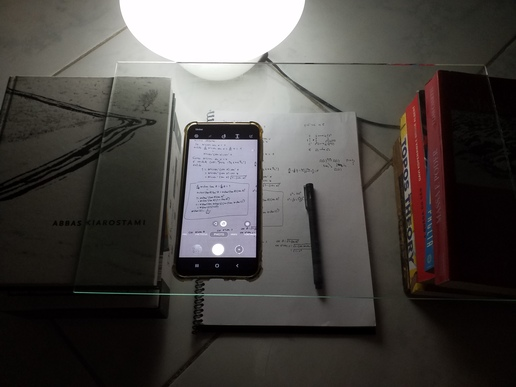
\includegraphics[height=2.5cm]{2020-1-C2/celular_apoiado_no_vidro_2.jpg}$$

\newpage

Eu pus na página do curso vários links sobre como escrever matemática
claramente - procure em ``Alguns textos pra discutir a correção das
provas''. Este aqui é o mais importante de todos:

\ssk

\url{http://angg.twu.net/LATEX/material-para-GA.pdf#page=5}

\ssk

Eu recomendo que as pessoas que ficaram em VS discutam entre si, tanto
pra tirar dúvidas quanto pra ensaiar pedaços das suas apresentações e
ver se estão encontrando modos claros de apresentar o material dos
seus trabalhos. Pra incentivar isso eu vou fazer o seguinte:

\ssk

{\sl Perguntas feitas no grupo do Telegram serão respondidas com muito
  mais boa vontade do que perguntas feitas em privado.}

\msk

Sugiro que a discussão seja feita no grupo do Telegram da turma de de
tarde, e que as pessoas da turma de de manhã entrem no grupo da turma
de de tarde pra participar.

% \newpage
% 
% {\bf Sobre o critério de avaliação}
% 
% \ssk
% 
% Eu tenho notas manuscritas de como eu apresentaria os assuntos deste
% trabalho em aula, e para praticamente cada uma das figuras e dos
% sinais de ``='' dessas notas eu tenho uma noção clara de quais são as
% ``habilidades e competências'' necessárias pras pessoas entenderem bem
% aquela figura ou aquele passo, e tenho exercícios pra ajudar as
% pessoas a entenderem cada passo difícil. Essas notas são bagunçadas
% demais e são secretas (!!!), mas vou usá-las como uma espécie de lista 
% 
% 
% ... não vou mostrá-las pra ninguém mas vou
% usá-las como 




\newpage

{\bf Área do pedaço de pizza}

% (find-latexscan-links "C2" "20201213_area_fatias_pizza")
% (find-xpdf-page "~/LATEX/2020-1-C2/20201213_area_fatias_pizza.pdf")
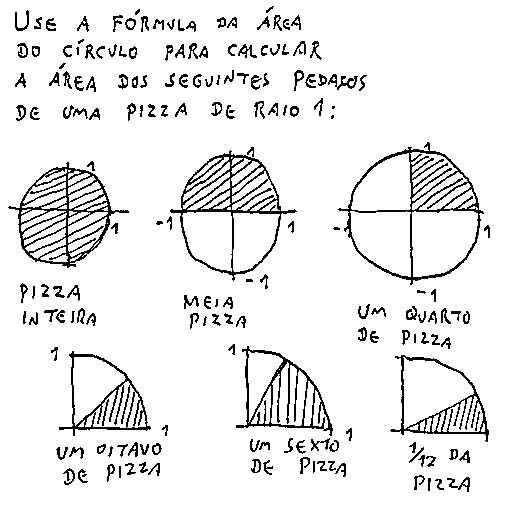
\includegraphics[height=7cm]{2020-1-C2/20201213_area_fatias_pizza.pdf}

\newpage

{\bf Calculando algumas áreas em função de $θ$}

% (find-latexscan-links "C2" "20201213_area_em_funcao_de_theta")
% (find-xpdf-page "~/LATEX/2020-1-C2/20201213_area_em_funcao_de_theta.pdf")
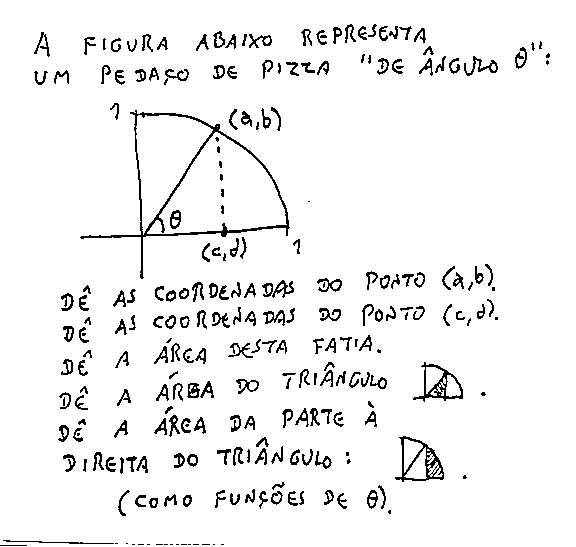
\includegraphics[height=7cm]{2020-1-C2/20201213_area_em_funcao_de_theta.pdf}

\newpage

{\bf Calculando algumas áreas em função de $x$}

% (find-latexscan-links "C2" "20201213_area_em_funcao_de_x")
% (find-xpdf-page "~/LATEX/2020-1-C2/20201213_area_em_funcao_de_x.pdf")
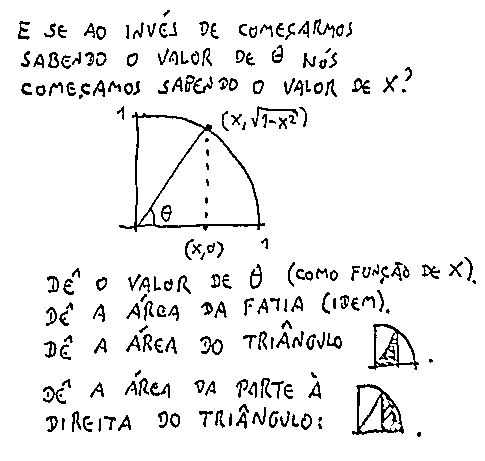
\includegraphics[height=7cm]{2020-1-C2/20201213_area_em_funcao_de_x.pdf}

\newpage

Agora represente graficamente
%
$$\begin{array}{r}
  \D \Intx{0}{0}{\sqrt{1-x^2}}, \\
  \D \Intx{0}{\frac12}{\sqrt{1-x^2}}, \\
  \D \Intx{0}{\frac{\sqrt2}2}{\sqrt{1-x^2}}, \\
  \D \Intx{0}{\frac{\sqrt3}2}{\sqrt{1-x^2}}, \\
  \D \Intx{0}{1}{\sqrt{1-x^2}}, \\
  \end{array}
$$

\newpage

e use o que você aprendeu nos slides anteriores pra dar uma fórmula

que calcula
%
$$\Intx{0}{b}{\sqrt{1-x^2}}$$

para qualquer valor de $b$ em $0≤b≤1$.

\msk

{\bf Dê um nome para esta sua fórmula.}

\msk

Teste-a para $b=0$, $b=1/2$, $b=\sqrt2/2$, $b=\sqrt3/2$, $b=1$.


\newpage

{\bf Por substituição trigonométrica}

Agora calcule 
%
$$\intx{\sqrt{1-x^2}}$$

por substituição trigonométrica.

{\bf Dê um nome para a fórmula que você obteve.}

\msk

Você provavelmente vai precisar de duas

identidades trigométricas ``clássicas'':

$(\cosθ)^2 = \frac12(1+\cos2θ)$ e

$\sen2θ = 2\senθ\cosθ$

\msk

O mini-teste 2 vai ter um método fácil de deduzir

estas identidades trigonométricas e várias outras.


\newpage

{\bf Por substituição trigonométrica}

\ssk

Use a fórmula que você obteve na página anterior para calcular
%
$$\Intx{0}{b}{\sqrt{1-x^2}}$$

Teste-a para $b=0$, $b=1/2$, $b=\sqrt2/2$, $b=\sqrt3/2$, $b=1$ e veja

se ela dá os mesmos resultados que o argumento geométrico.





\GenericWarning{Success:}{Success!!!}  % Used by `M-x cv'

\end{document}

% (find-vscan-links "2020-1-C2-VS")

 (eepitch-shell)
 (eepitch-kill)
 (eepitch-shell)
# (find-fline "~/2020.1-C2/")
# (find-fline "~/LATEX/2020-1-C2/")
# (find-fline "/tmp/")
cd /tmp/
for i in *.jpg; do echo f $(basename $i .jpg); done

f () { rm -fv $1.png $1.pdf; djvuize $1.pdf }
f () { rm -fv $1.png $1.pdf; djvuize WHITEBOARDOPTS="-m 1.0" $1.pdf; xpdf $1.pdf }
f () { rm -fv $1.png $1.pdf; djvuize WHITEBOARDOPTS="-m 0.5" $1.pdf; xpdf $1.pdf }
f () { rm -fv $1.png $1.pdf; djvuize WHITEBOARDOPTS="-m 0.25" $1.pdf; xpdf $1.pdf }
f () { cp -fv $1.png $1.pdf       ~/2020.1-C3/ }
f () { cp -fv        $1.pdf ~/LATEX/2020-1-C3/ }
f () { cp -fv $1.png $1.pdf       ~/2020.1-C2/
       cp -fv        $1.pdf ~/LATEX/2020-1-C2/
       cat <<%%%
% (find-latexscan-links "C2" "$1")
%%%
}

f 20201213_area_em_funcao_de_theta
f 20201213_area_em_funcao_de_x
f 20201213_area_fatias_pizza


cd /tmp/
FILE0=celular_apoiado_no_vidro.jpg
FILE1=celular_apoiado_no_vidro_2.jpg

convert $FILE0 -resize 12.5\% $FILE1
laf $FILE0 $FILE1
cp -v $FILE1 ~/LATEX/2020-1-C2/
# (find-fline "/tmp/celular_apoiado_no_vidro_2.jpg")

%  __  __       _        
% |  \/  | __ _| | _____ 
% | |\/| |/ _` | |/ / _ \
% | |  | | (_| |   <  __/
% |_|  |_|\__,_|_|\_\___|
%                        
% <make>

 (eepitch-shell)
 (eepitch-kill)
 (eepitch-shell)
# (find-LATEXfile "2019planar-has-1.mk")
make -f 2019.mk STEM=2020-1-C2-VS veryclean
make -f 2019.mk STEM=2020-1-C2-VS pdf

% Local Variables:
% coding: utf-8-unix
% ee-tla: "c2m201vs"
% End:

